\documentclass[sigconf,nonacm,prologue,table]{acmart}
\usepackage{listings}

%% labels
%% sections:    "sec"
%% definitions: "def"
%% equations:   "eq"
%% figures:     "fig"
%% tables:      "tab"

%% packages
\usepackage{amsmath}
% \usepackage{pgfplots}
\usepackage{subcaption}
\usepackage{commath}
\usepackage[utf8]{inputenc}
% \usetikzlibrary{positioning, arrows.meta, shapes, calc}
%% \usepackage{tikz}
\usepackage{graphicx}
\graphicspath{ {../docs/} }
\usepackage{afterpage}

\pagenumbering{arabic}

%% hide ACM reference
\settopmatter{printacmref=false}

%% hide copyright
\renewcommand\footnotetextcopyrightpermission[1]{}

%% \pagestyle{plain}
\settopmatter{printfolios=true}

% \numberwithin{equation}{section}

% \theoremstyle{definition}
% \newtheorem{definition}{Definition}

% \theoremstyle{remark}
% \newtheorem*{remark}{Remark}

\newcommand{\dshares}{\textsc{Dinari} d\textsc{Shares} }

\begin{document}
\title{Dinari Securities Backed Tokens (dShares) v1 [Draft]}
\subtitle{June 2023}
\date{June 2023}

\author{Jake Timothy}
\affiliation{}
\email{jake@dinari.com}

\begin{teaserfigure}
\caption*{
    \hspace{\textwidth}
    }
\end{teaserfigure}

\renewcommand{\shortauthors}{Timothy}

\begin{abstract}

    Dinari Securities Backed Tokens (dShares) is a trusted bridge from the existing financial system to the new world of decentralized finance. Such a bridge is necessary to enable a more accessible, transparent, and efficient system for the world’s quadrillions of dollars in spot and derivatives trading. 
    
    The \dshares protocol defines a standard for tokens backed 1-to-1 by existing publicly traded securities and order processor smart contracts that process primary purchases and sales of those tokens.  A set of automated operators maintain the 1-to-1 backing while filling those orders. As orders are submitted to \dshares, order processor operators run by Dinari automatically rebalance the underlying securities vault accounts, working with multiple clearing services, to maintain at least 100\% backing of the outstanding token issuance.

    \dshares are redeemable through sell orders for the current value of the underlying shares held in the vault accounts.

\end{abstract}

\maketitle

\section{Introduction}
\label{sec:introduction}

\dshares is designed to maximize interoperability with decentralized finance while maintaining security. This enables users to submit and manage orders manually and programmatically.

\section{The Tokens} 
\label{sec:Tokens}

\dshares are ERC-20 compliant and compatible with standard decentralized financial applications.

\subsection{Transfer Restrictions}

\dshares have a transfer blacklist feature for enforcing OFAC, AML, and other account security requirements. A blacklisted account will not be able to send or receive tokens.

\dshares deploys one TransferRestrictor per issuing jurisdiction. All tokens backed by assets issued in one jurisdiction share a transfer restrictor. Tokens backed by assets issued in another jurisdiction may have different security requirements.

\subsection{Voting}

In order for the \dshares to trade freely without more onerous transfer restrictions, Dinari holds back shareholder voting rights from tokenholders.

Since the underlying securities are held by Dinari in vault accounts, the total amount of shares would need to vote together. In order to prevent unknown actors from accumulating voting power, tokenholders would register in order to cast their vote. We expect that for any shareholder vote, a small percentage of the overall token supply would register, complete a KYC process, and participate in voting. This would result in a small amount of tokens directing a potentially large block of voting power. For the time being, we have decided not to have token holders direct the Vault’s shareholder voting decisions.

\subsection{Dividends and Distributions}

\dshares holders earn dividends from the underlying asset if that asset issues dividends. When dividends are announced for the underlying security, token holdings are snapshot at the block corresponding to the announced distribution time. Distributions are deposited into a claim contract in USDC where they are availabe for accounts to withdraw up to their distribution amount for period of time.

\subsection{Proof of Reserves}

\dshares maintains 1-to-1 backing in real time by determining if any security purchases are necessary and executing those purchases for every order request. When a request is received, if the current reserves are not sufficient to maintain at least 100\% backing, purchases of the the underlying security are initiated. Dinari publishes the latest order activity in real time and current vault balances at regular intervals. Dinari vault accounts are held by a custodian and audited at random times by a third party to verify the integrity of accounting and reporting. 

\section{Order Processors}
\label{sec:Processors}

The \dshares protocol operates like a bridge. Calls to contracts inheriting from OrderProcessor emit Orders. Orders emitted from official OrderProcessor deployments are picked up by Dinari's fulfillment service, which executes a brokerage order through a clearing service when necessary. The clearing service then settles the order and notifies the fulfillment service. The fulfillment service in turn submits a fill to the OrderProcessor and dShares are minted or burned to the order recipient, along with any payment token transfers for order payment or distribution of proceeds. Different order processing logic can be implemented. The Order specification supports market and liimit order types.

\dshares v1 has implemented
\begin{itemize}
    \item An escrow locked market buy processor
    \item An escrow locked market sell processor
    \item An escrow unlocked market buy processor
\end{itemize}

An example order processing sequence diagram is shown in Figure~2.

\begin{figure}
    \centering
    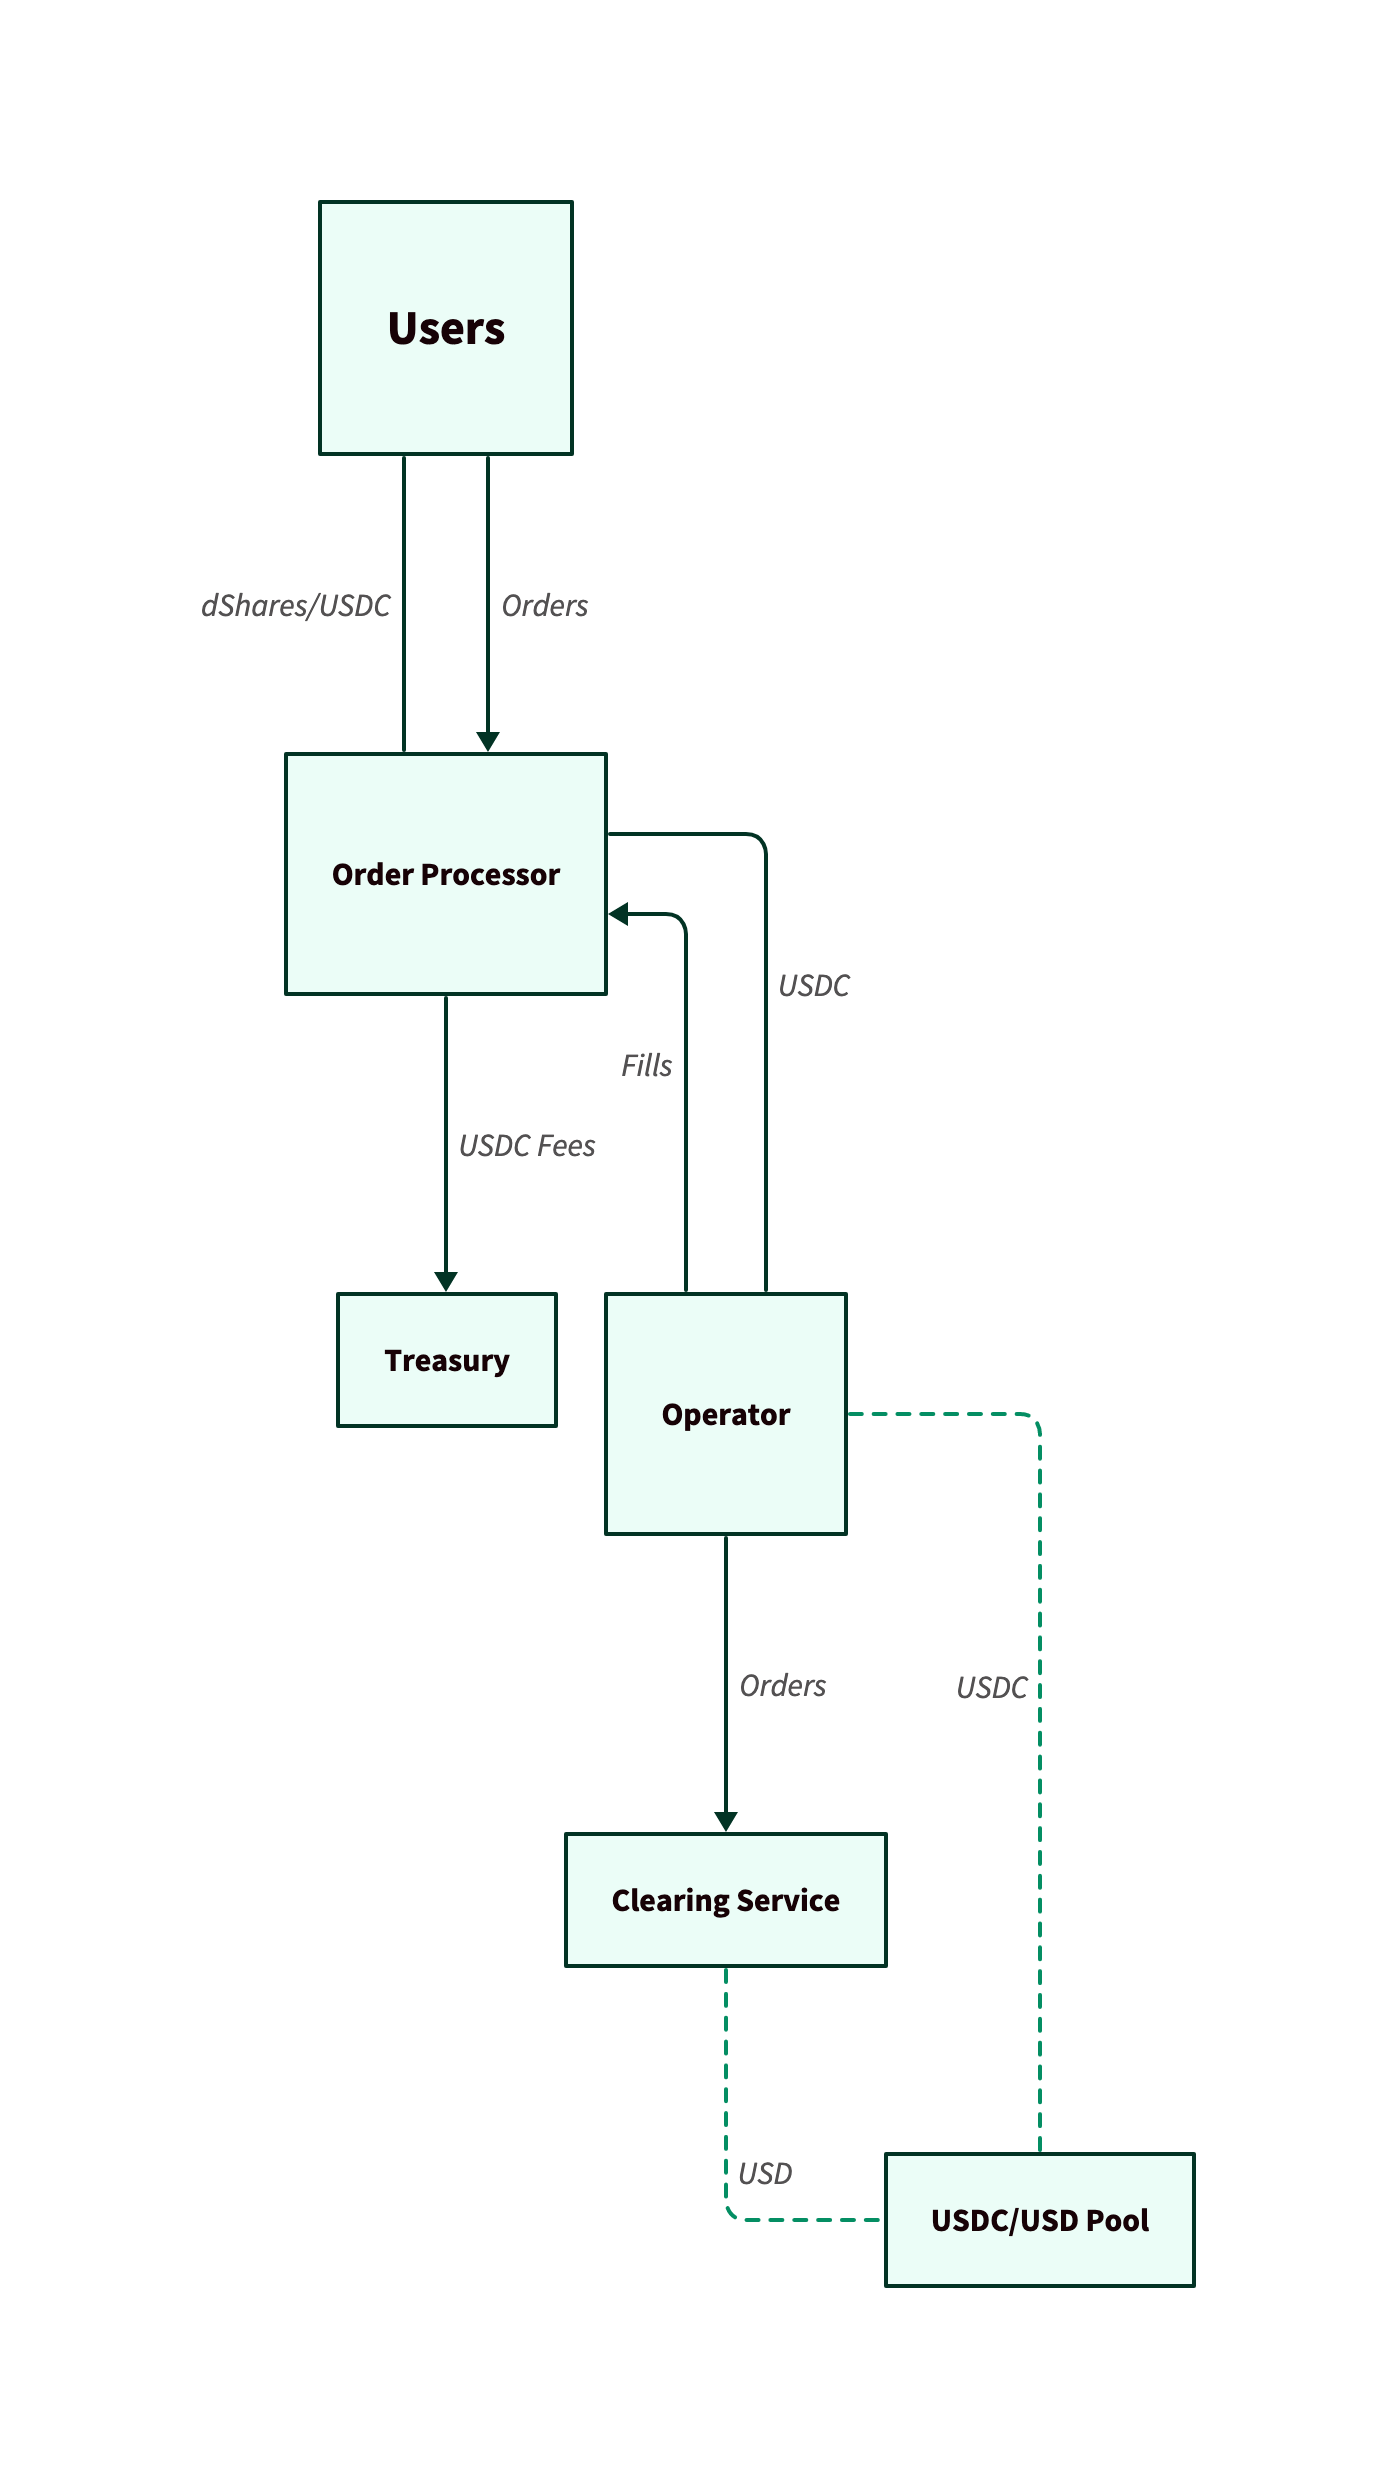
\includegraphics[width = 0.5\textwidth]{flow.d2}
    \caption{Order and Asset Flow}
    \label{fig:flow}
\end{figure}

% replace with ref
Figure~1 shows the flow of orders and assets through the system. Asset flow is bidirectional as needed. Submitted orders specify an asset token (the dShare) and a payment token (e.g. USDC). A buy order takes payment token and gives dShares when filled. A sell order takes dShares and gives payment token when filled. dShares are minted or burned by the order processor as the order is filled. 

Order processor operators are responsible for managing their payment token and fiat liquidity to ensure that orders can be filled.

\subsection{Fees}

OrderProcessor fees include a flat per-order fee and a percentage fee rate applied to the order amount. These fees are taken from the payment token, from the payment amount for buy orders, or from the proceeds of the sale for sell orders.

\section{Summary}

As a transparent, accessible, and interoperable standard for Securities Backed Tokens, \dshares enables a core building block for a more fair and open financial system.

% \bibliographystyle{ACM-Reference-Format}
% \bibliography{whitepaper}

\section*{Disclaimer}

This paper is for general information purposes only. It does not constitute investment advice or a recommendation or solicitation to buy or sell any investment and should not be used in the evaluation of the merits of making any investment decision. It should not be relied upon for accounting, legal or tax advice or investment recommendations.  This paper reflects current opinions of the authors. The opinions reflected herein are subject to change without being updated. 

\newpage
\phantom{.}
\afterpage{
\begin{figure}
    \centering
    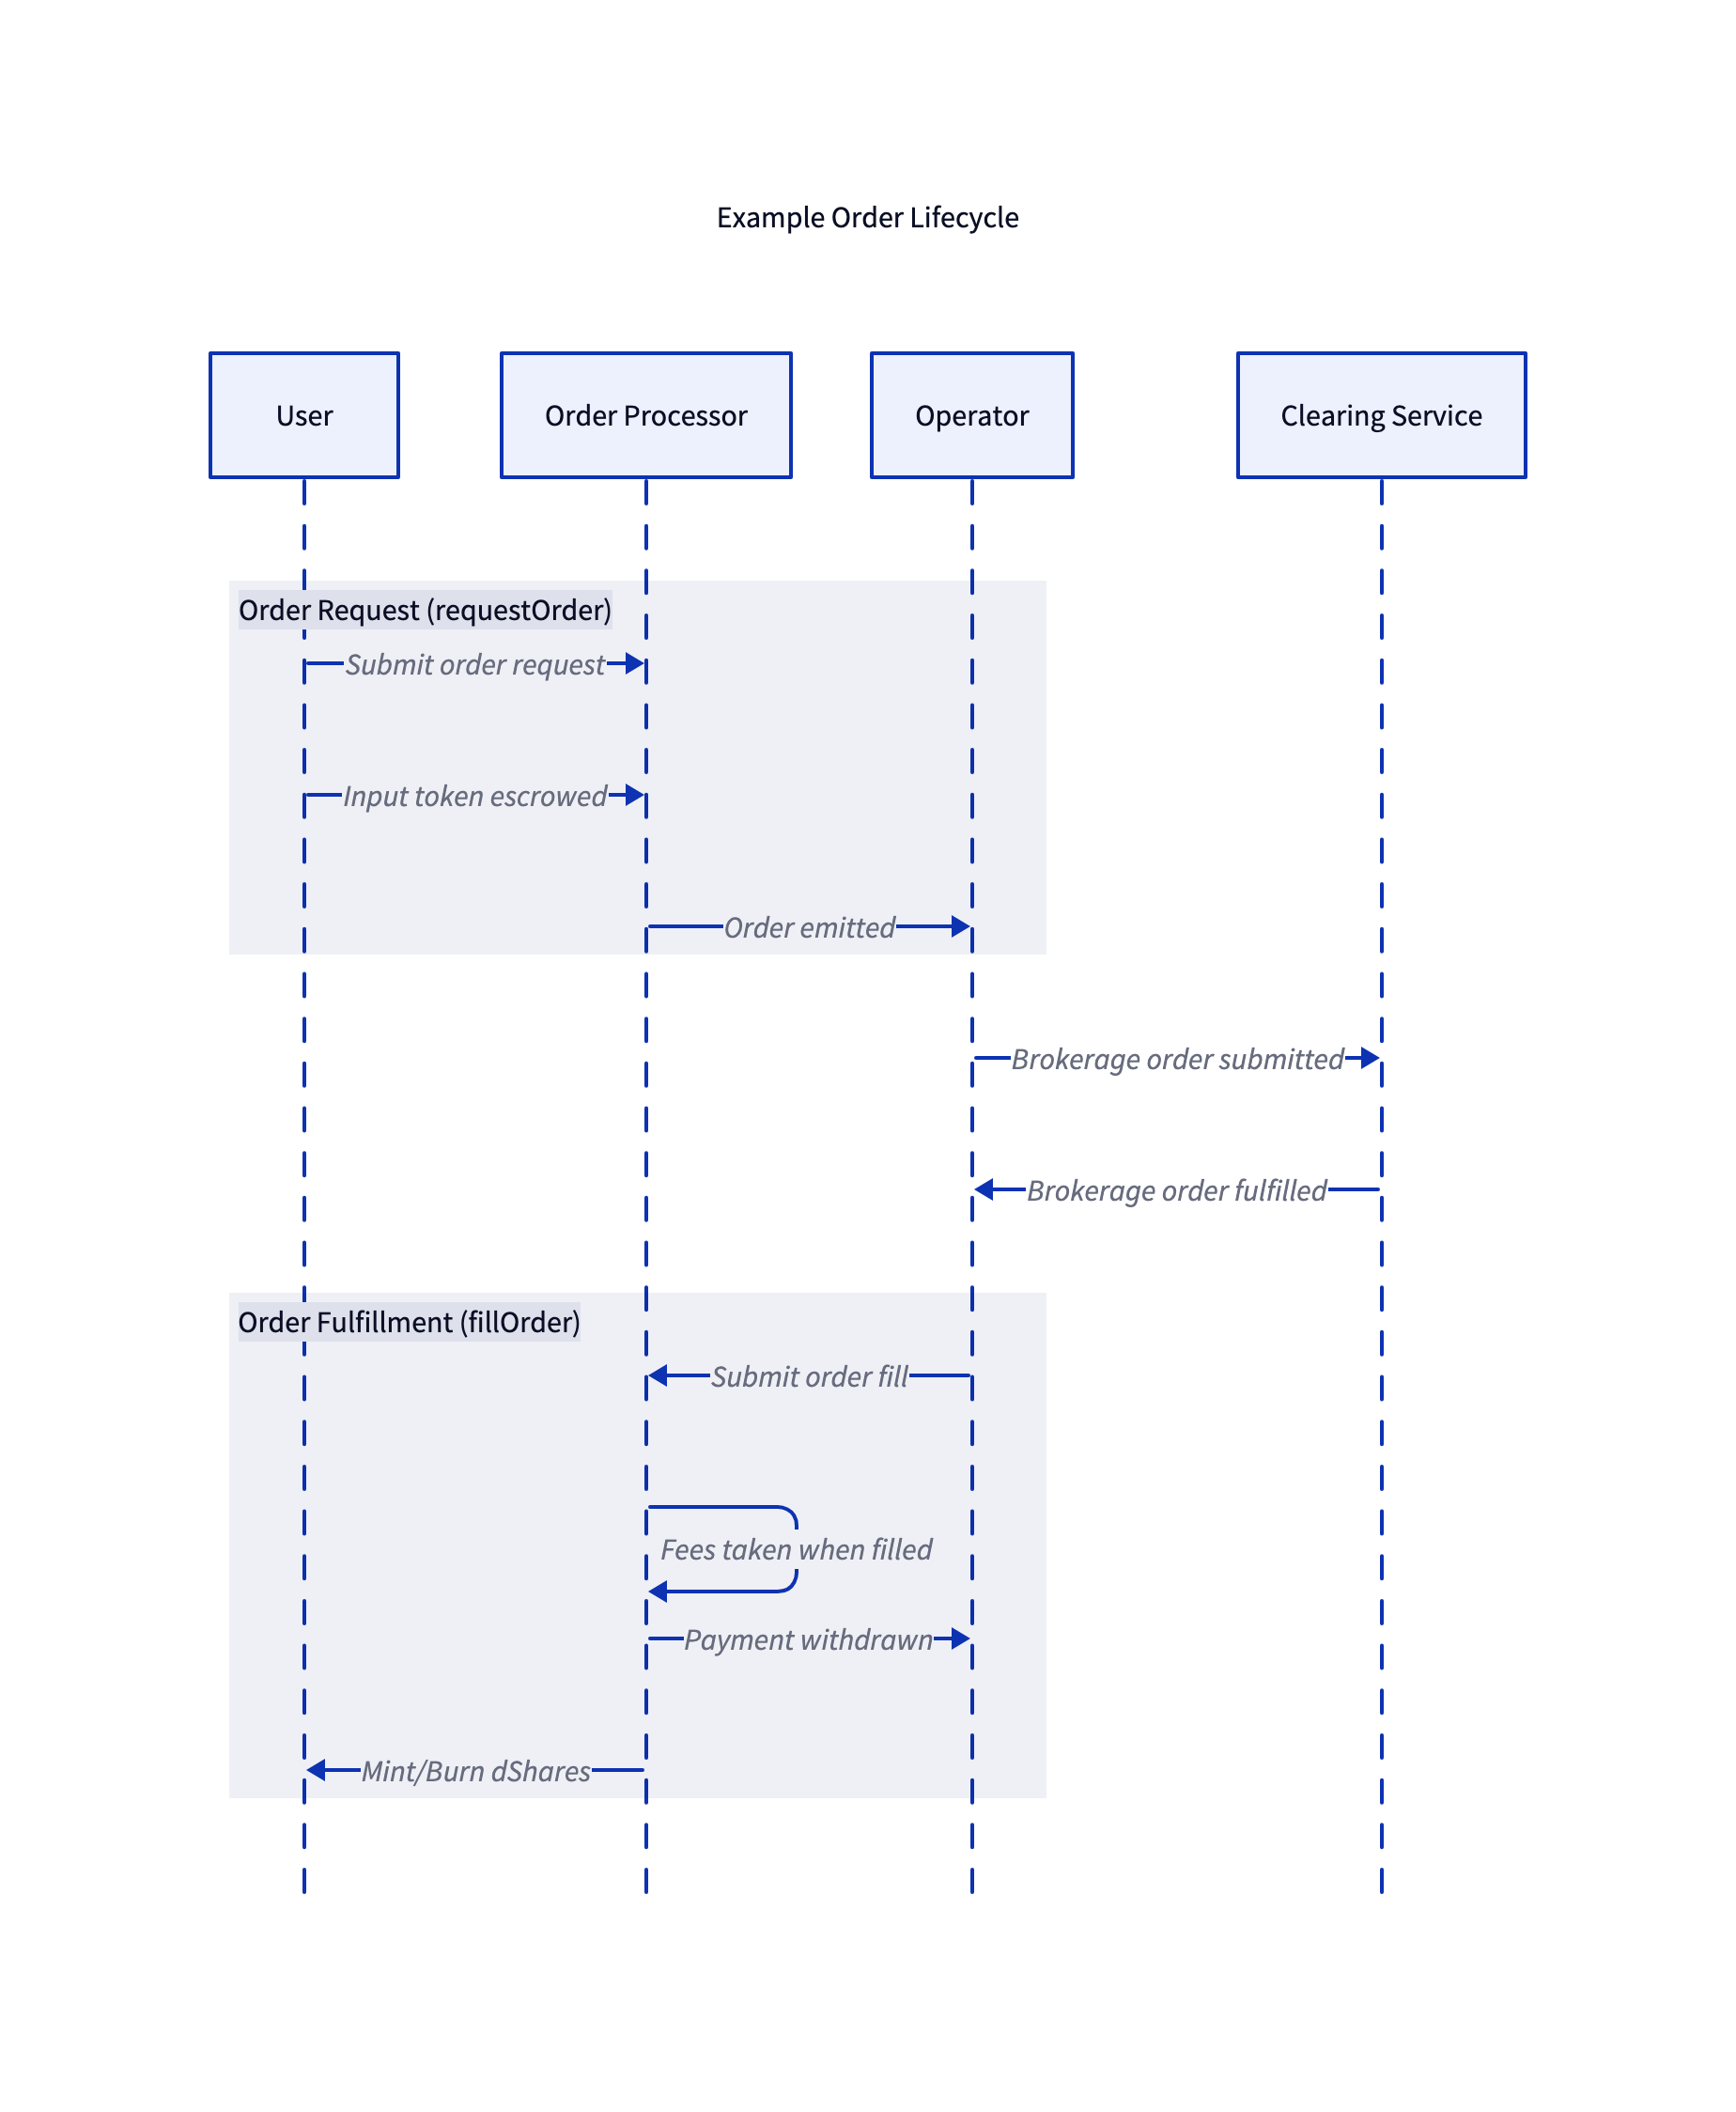
\includegraphics[width = \textwidth]{order-lifecycle.d2}
    \caption{Order Processing Example}
    \label{fig:order-processing}
  \end{figure}
  \clearpage
  }

\end{document}
